\section{A Substituição do trabalho pelo capital}

O modelo neoclássico de crescimento sustenta que se os fatores de produção, capital e trabalho têm rendimentos decrescentes.
\citeonline{piketty2013capital} relata que enquanto a taxa de retorno do capital for superior à taxa de crescimento, a parcela do capital na renda aumentará.
Então, se o retorno do capital for mais alto do que o crescimento da economia, a renda dos que têm capital aumentará mais do que a renda dos que vivem do trabalho.
Assim, os indivíduos que possuem capital apropriam-se de quase toda a renda, tornando altamente improvável que se possa acumular capital a partir da renda apenas do trabalho.
Logo, a sociedade desigual, onde não há risco de perder a fortuna herdada, nem esperança de enriquecer, é seguramente incompatível com a democracia, conforme ilustra a Figura~\ref{fig:concentracao-renda}. 


\begin{figure}[!ht]
    \centering
    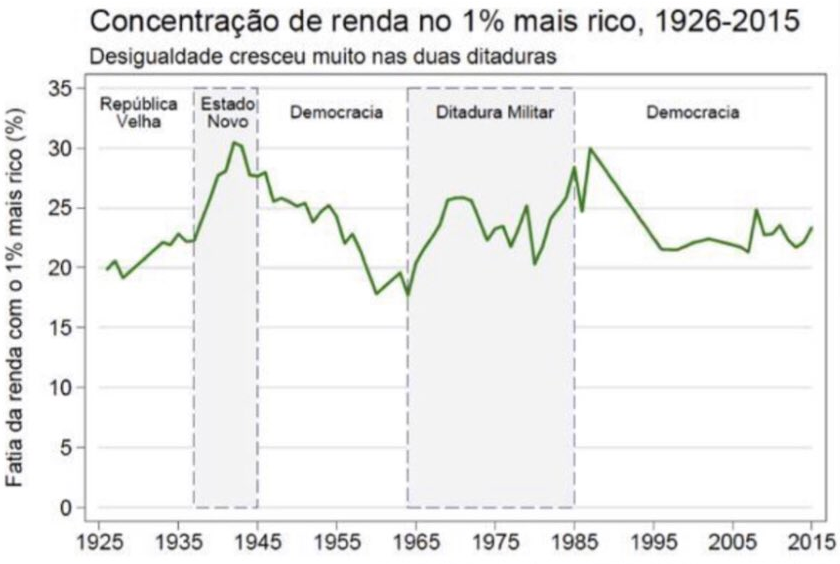
\includegraphics[width=.7\linewidth]{img/concentracao-renda.png}
    \caption{Concentração de renda no Brasil durante 1925 à 2015.
    Adaptado de \citeonline{souza2016desigualdade} a partir de tabulações de dados tributários e das Contas p.221}
    \label{fig:concentracao-renda}
\end{figure}
